\chapter{Game Development}
\label{chap:game_development}

\section{Fasi dello sviluppo}

I lavori sul progetto ``The Magic Lantern'' sono iniziati tra Gennaio e Febbraio 2014 ed i primi meeting con l'azienda sono serviti per spiegare i retroscena del progetto e il documento di game design iniziale.
Al secondo meeting è stata definitiva una timeline per l'intero lavoro, in buona parte rispettata. 

%La timeline ha previsto una divisione del lavoro in due macro sezioni, dove in %ognuna delle quali sono stati portati a termine vari sotto-fasi ed obiettivi:
La timeline ha previsto una divisione del lavoro in due macro-sezioni, ognuna delle quali a sua volta costituita da fasi ed obiettivi differenti:

\begin{itemize}

\item Pre Production: periodo stimato (Febbraio-Marzo)

\begin{itemize}
\item High Concept revision: all'inizio è servito rivedere il concept iniziale, recepire i feedback ricevuti come risposta alla partecipazione al bando Creative Europe (per la quale il progetto si era precedentemente iscritto) e quindi riformulare, tramite varie sessioni di brainstorming, un nuovo concept.
\item Pitch: rielaborato il concept, si è spiegato tutto in un breve pitch, per definire bene i nuovi intenti di design.
\item Concept art revision: oltre al concept di gameplay si è fatto un concept anche a livello artistico.
\item Game Design Document updating: una volta approvato il pitch e le varie revisioni, l'obiettivo è stato quello di riscrivere il documento di game design.
\item Prototyping: definito il documento di design, si è creato un prototipo che confermi in prima battuta le scelte di design prese. Questi ultimi 2 step sono stati ripetuti più volte.
\end{itemize}

\item Production: periodo stimato (Aprile-Luglio)

\begin{itemize}
\item Game Design: una volta scelto il Game Design definitivo dalla fase precedente, questo è stato rivisto e ulteriormente raffinato.
\item Development: a questo punto, lo sviluppo vero e proprio della demo definitiva è partito.
\item Level Design: buona parte del lavoro, della fase di production, è stato dedicato al level design, in quanto, una volta creato un gameplay di base, è servito studiare come farlo fruire al giocatore.
\item Art production: a questo punto è stato necessario il supporto dal reparto grafico al fine di ``colorare'' e ``riempire'' il mondo di gioco. In genere gli artisti forniscono concept al resto del team al fine di fornire anche nuove idee per livelli e ambientazioni varie. In questo caso specifico, il reparto artistico ha fornito gli asset indispensabile per rendere il gioco chiaro e minimamente godibile.
\item Audio production: per ogni sezione di gioco è stato inserito il relativo audio, al fine di trasmettere le sensazioni volute al player.
\item First Playable: dopo aver tenuto conto di tutti i focus precedenti, si è passati alla creazione della prima versione giocabile della demo.
\item Testing alpha version: finalizzata la demo giocabile, questa va testata tramite il pubblico target, quindi vanno analizzati i risultati e i feedback raccolti.
\end{itemize}

\end{itemize}

%La fase di Pre-Production è stata, in buona parte, rispettata. 
La timeline della fase di Pre-Production è stata, in gran parte, rispettata.
L'inizio dei lavori per la fase di Production, invece, è stata ritardato di qualche settimana per via delle vacanze Pasquali e altre rielaborazioni varie che hanno riguardato gli ultimi due focus del pre-production (Game Design Document e Prototyping), in quanto è stato necessario provare più volte versioni dei design pensati (come è solito succedere per ogni videogame che attraversa questa fase). Qui sono state fatte alcune prove di gameplay, tentando varie combinazioni di comandi per l'uso dello strumento centrale del gioco, la Lanterna Magica. Come già detto nel capitolo di Game Design (\ref{chap:game_design}), si è inoltre scelto di concentrare il gioco soprattutto sulle meccaniche intorno alla Lanterna, piuttosto che dare un uguale peso ad altre tecnologie del pre-cinema, se così non fosse stato, si sarebbero create troppe combinazioni e la complessità del gioco si sarebbe elevata troppo, considerati anche il tempo e i mezzi a disposizione. Si è scelto quindi di utilizzare le altre tecnologie in altri modi, come per esempio mini livelli o comunque sezioni limitate di gioco. In generale, questa fase ha visto un largo studio dello stato dell'arte dei giochi di interesse per il nostro studio, giochi sia di tipo Serious Game sia di tipo platform e puzzle. Si è quindi provato a prendere spunto dai pattern più famosi al fine di rendere il gioco il più comprensibile possibile.

La fase di Production, iniziata a fine Aprile, ha visto una porzione enorme di tempo dedicata al level design. Non è stato facile definire un livello di difficoltà per il pubblico target ed in generale per il giocatore. In questa fase ci si è scontrati con dei veri problemi di design, e si è cercato di capire come una meccanica andrebbe fornita al player. Per fare ciò, ci si è ispirati in parte anche ai giochi esposti nella sezione dello stato dell'arte (\ref{chap:stato_dell_arte}). Dopo la prima fase dei lavori, durante la quale sono stati usati dei placeholder, abbiamo usufruito del supporto del reparto grafico per rendere il gioco più chiaro e adatto per un generico pubblico, assistenza giunta nel mese di Giugno (nonostante la timeline prevedeva il periodo tra Aprile e Maggio). A causa di vari ritardi, come quello del supporto grafico, la continua re-implementazione dei livelli finali e la scelta delle modalità di fruizione dei contenuti Serious, la fase di Production (della demo) non si è potuta concludere a Luglio, come stabilito. Questo anche perché si è riusciti a portare a termine solo il primo round di testing, mentre per questioni di completezza sarebbe stato necessario farne almeno un secondo per apportare le modifiche necessarie in base ai feedback ricevuti durante il primo round, e quindi capire valutare l'efficacia dei cambiamenti applicati. Ovviamente, prima dei test esterni, sono state svolte varie sedute di testing interno all'azienda, per capire se il prodotto fosse pronto per un pubblico esterno.


\section{Strumenti}

The Magic Lantern è stato implementato tramite il game engine Unity3D versione 5.1.1.f1 (\url{https://unity3d.com}) usando prevalentemente il linguaggio di programmazione C\#. Unity3d è un game engine che fornisce un editor molto semplice e potente, col quale si può familiarizzare anche in poche ore, e con il quale si possono ottenere ottimi risultati pur con una minima conoscenza di computer graphic e programmazione. Esistono moltissimi tutorial sul web che trattano di Unity3D, e la community è molto attiva, ciò semplifica ancor di più l'apprendimento dello strumento.

Come sistema di versioning è stato utilizzato Git (\cite{github}), tramite il programma SourceTree che fornisce una interfaccia grafica molto facile da utilizzare.

E' stato utilizzato inoltre, come strumento di team management e comunicazione interna, il programma Asana (\cite{asana}). Questo è uno strumento molto utile per assegnare task e fissare scadenze, elementi essenziali per lavorare efficientemente in team.


\section{Logica implementativa di gameplay}

\section{Controller del player}
\label{sec:player_movements}

Il videogioco si basa su classiche meccaniche \textit{platform}, il personaggio deve perciò essere capace di correre, saltare, salire scale. La classe \textit{playerMovements} si occupa appunto di gestire questi comportamenti.
Il player è gestito da una macchina a stati, mostrata in Figura~\ref{fig:development_player_stati}, che ne descrive lo stato attuale ed eventuali transizioni.

\begin{figure}%[h]
	\centering
	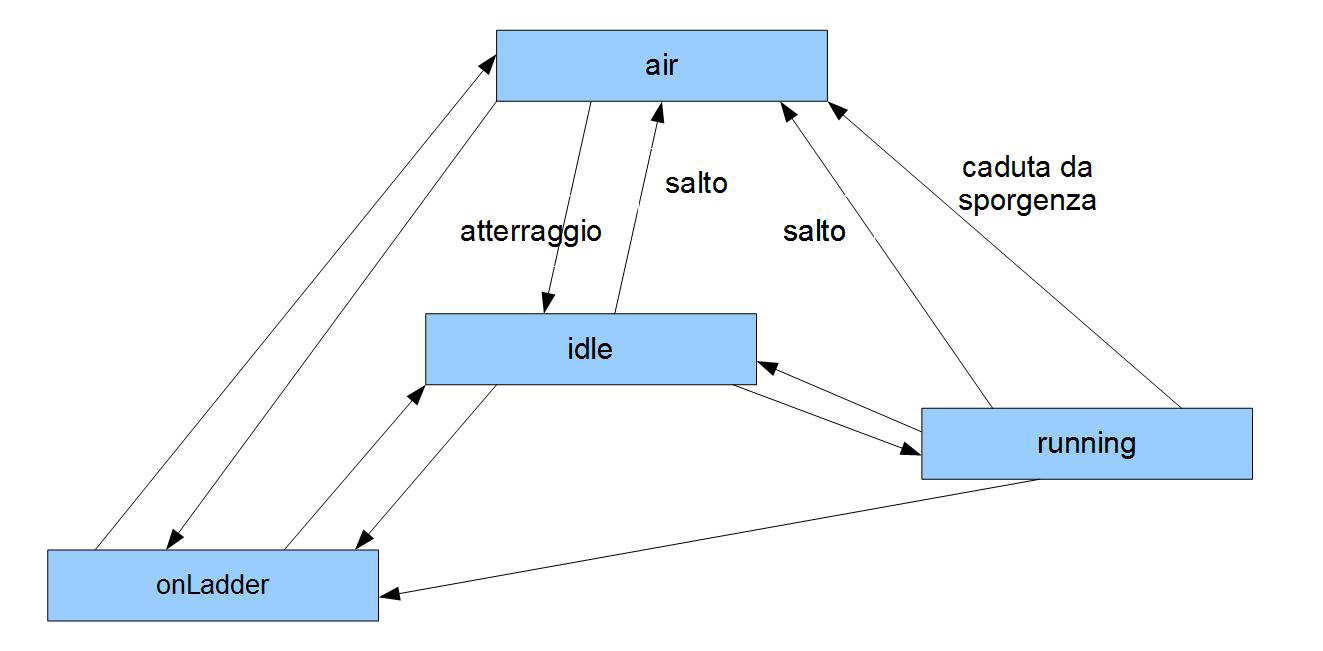
\includegraphics[width= 0.9\columnwidth]{images/development/player.jpg}
	\caption{Diagramma con gli stati del player.}
	\label{fig:development_player_stati}
\end{figure}

La classe, in primo luogo, si occupa di controllare se il player stia toccando terra o meno. Nel primo caso, il giocatore può utilizzare i tasti direzionali per cambiare il suo stato da \textit{idle} a \textit{running}. Inoltre, se l’attuale direzione risulta opposta a quella di movimento, il cambio di stato è preceduto da un’inversione di scala del personaggio.
Oltre alle situazioni in cui questo tocchi terra, il player può trovarsi nello stato di \textit{air}. In questa situazione i tasti direzionali possono essere utilizzati per controllare la caduta, in maniera limitata rispetto a quanto avviene a terra.
Lo stato di \textit{air} può essere raggiunto in due modi:

\begin{itemize}
	\item Spiccando un salto mentre è verificata la condizione di ground. In questo caso viene applicata una forza positiva lungo l’asse y.	
	\item Lasciandosi cadere da una sporgenza.
\end{itemize}

Raggiungendo lo stato \textit{air} il player mantiene la sua velocità lungo l’asse x, che può essere in parte limitata tramite i tasti direzionali, ma è soggetto ad una forza di gravità che lo spinge verso il basso.
La gravità, secondo canoni tipici dei giochi platform, è triplicata rispetto a quella standard, l’accelerazione di caduta risulta perciò molto enfatizzata. La velocità è comunque limitata da un valore massimo.
Oltre agli stati citati, esiste quello di \textit{onLadder}, questa particolare situazione descrive il personaggio mentre questo si trova ad utilizzare un scala. Il giocatore può decidere di scendere o salire attraverso i tasti direzionali. Lo stato può essere raggiunto sia quando il player è a terra, che quando si trova nella situazione \textit{air}, semplicemente premendo un tasto direzionale, lungo l’asse verticale, nei pressi di una scala.
Per lasciare lo stato di \textit{onLadder} esistono più modi:

\begin{itemize}
	\item Premendo un tasto direzionale lungo l’asse orizzontale. Viene impressa una piccola forza laterale al player, e questo passa allo stato di \textit{air}.	
	\item Raggiungendo la base della scala, se nella parte sottostante è presente un terreno, il personaggio la lascia, entrando nello stato ground, \textit{idle}.
	\item Raggiungendo la base della scala, se nella parte sottostante non è presente un terreno, il personaggio la lascia, entrando nello stato \textit{air}.
\end{itemize}

La classe \textit{playerMovements} è anche utilizzata come interfaccia dalle classi dell’\textit{AI} per richiamare metodi di movimento dei personaggi.

\section{Lanterna Magica e vetrini}

L’utilizzo della Lanterna Magica è la meccanica di gioco principale, questa permette di proiettare oggetti nell’ambientazione e modificare lo scenario di gioco.
Le classi \textit{MagicLantern} e \textit{MagicLanternGraphic} ne gestiscono interamente il comportamento.
\textit{MagicLantern}, classe derivata di \textit{Tool}, si occupa dello stato attuale della Lanterna e dei vari cambiamenti di stato in base all’input dell’utente.

\begin{figure}%[h]
	\centering
	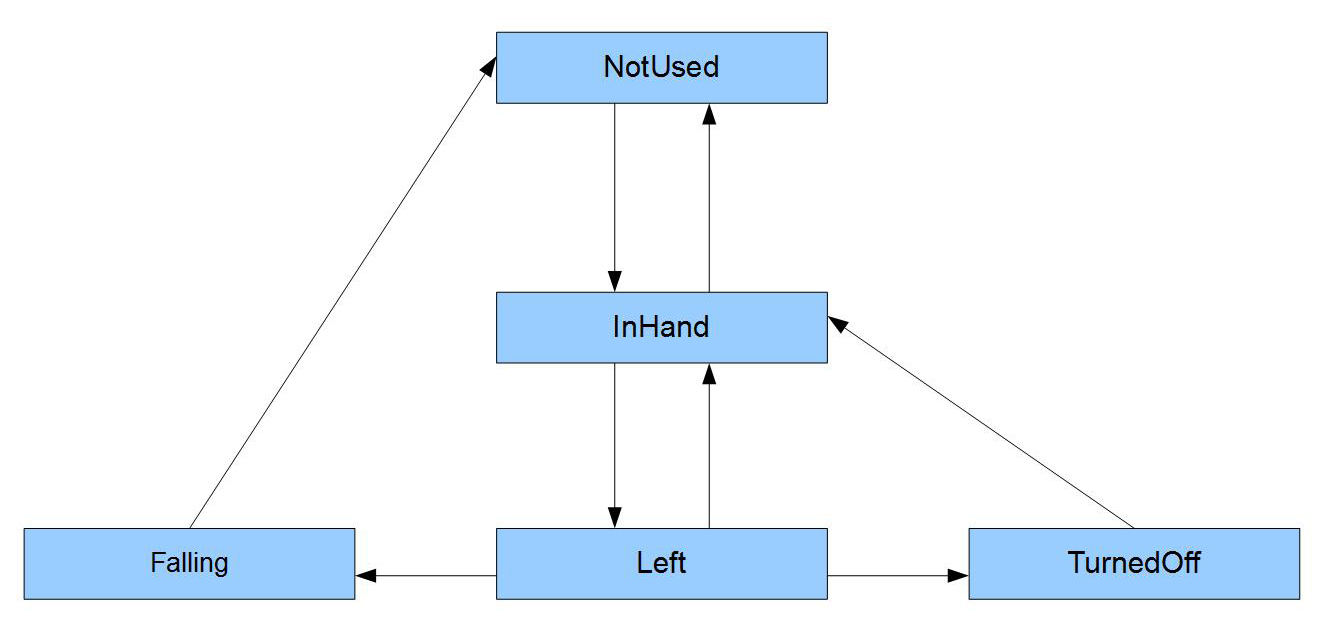
\includegraphics[width= 0.9\columnwidth]{images/development/lanterna.jpg}
	\caption{Diagramma con gli stati della Lanterna Magica.}
	\label{fig:development_lanterna_stati}
\end{figure}

Come mostrato in Figura~\ref{fig:development_lanterna_stati}, la Lanterna si può trovare nei seguenti stati:

\begin{itemize}
	\item \textit{\textbf{NotUsed.}} Non è utilizzata dall’utente e risulta non visibile a schermo
	\item \textit{\textbf{InHand.}} Il personaggio sta usando la Lanterna, viene quindi mostrata a schermo, sovrapposta al player, ed il giocatore può usare il puntatore per mirare, prima di rilasciare e creare la proiezione.
	\item \textit{\textbf{Left.}} Il giocatore ha mirato e lasciato la Lanterna a terra. Questa sta perciò proiettando.
	\item \textit{\textbf{TurnedOff.}} La Lanterna è stata toccata da un nemico che l’ha spenta. Questo stato non è attualmente utilizzato nel prototipo sviluppato, in quanto si è negata la possibilità al nemico di spegnere la Lanterna.
	\item \textit{\textbf{Falling.}} La Lanterna sta cadendo.
\end{itemize}

All’inizio della partita, il giocatore non possiede ancora la Lanterna Magica, il \textit{gameObject} con la classe \textit{MagicLantern} è quindi disabilitato. Al primo raccoglimento della Lanterna, questa si trova nello stato \textit{NotUsed}. Il giocatore può quindi iniziare a mirare e passare allo stato \textit{InHand}. In questo stato la Lanterna è figlia del player, quindi lo segue durante i suoi movimenti.
Il giocatore può continuare a mirare, ad esclusione degli stati \textit{air} ed \textit{onLadder} del player (Capitolo \ref{sec:player_movements}).
Al momento del rilascio del tasto utilizzato per mirare, la Lanterna viene lasciata a terra, raggiunge perciò lo stato \textit{Left} e la proiezione viene resa tangibile ed interagibile. Se, al momento del rilascio, il player si trovava negli stati non adatti alla proiezione, precedentemente specificati, la Lanterna raggiunge lo stato \textit{NotUsed}.
Dallo stato \textit{Left}, la Lanterna può tornare direttamente a quello \textit{InHand} se l’utente preme il tasto per mirare, oppure a \textit{TurnedOff}, se è raggiunta da un nemico, o \textit{Falling} se il terreno sottostante scompare.
Dallo stato \textit{Falling}, la Lanterna raggiunge direttamente quello \textit{NotUsed} dopo un breve intervallo temporale.

La classe \textit{MagicLantern}, a seconda dello stato attuale, invoca particolari metodi della classe \textit{MagicLanternGraphic}, che si occupa invece di gestire la grafica dell’oggetto.
Il puntatore viene utilizzato per mirare, durante queste fasi, la sagoma della proiezione segue il puntatore, attraverso una funzione di \textit{smoothing} che rende i movimenti più piacevoli. La direzione del raggio viene quindi calcolata dinamicamente sulla base delle posizioni del player e della proiezione.
\textit{MagicLanternGraphic} si occupa quindi anche di spegnere ed accendere la lanterna, oltre che di cambiare la grafica del raggio, in modo da mostrare coerentemente gli stati \textit{InHand} e \textit{Left}.


\section{AI e spawner}

Poiché il gioco prevede l'interazione con dei nemici, è stato necessario sviluppare una logica di AI. Essendo il comportamento designato per i nemici non molto complesso, si è scelto di utilizzare una macchina a stati come logica di base, evoluta in un secondo momento in una macchina a stati gerarchica.

E' possibile vedere un Class Diagram che rappresenta l'implementazione usata:

\begin{figure}[h]
\centerline{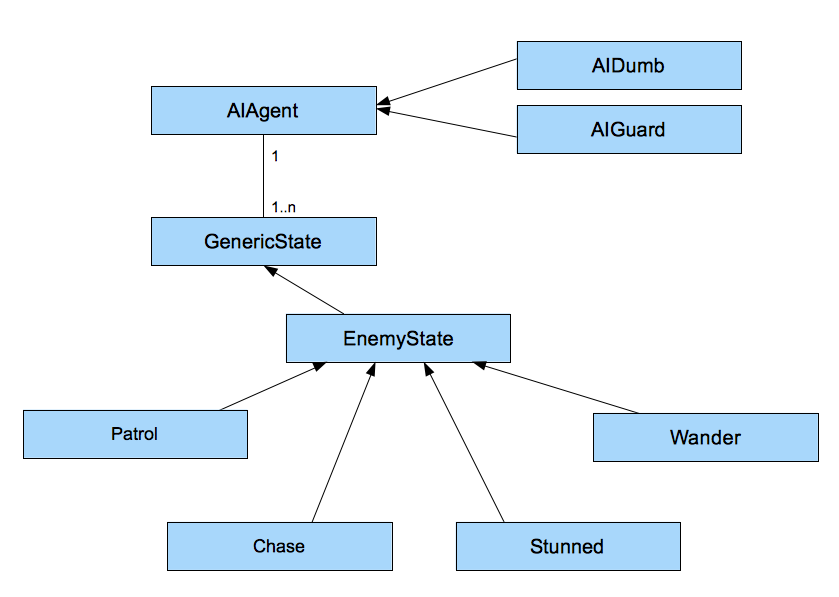
\includegraphics[scale=0.45]{images/development/classdiagramAI.png}}
\caption{Class Diagram della AI usata.}
\label{fig:classdiagramAI}
\end{figure}

Il funzionamento di questa macchina a stati dà la possibilità di gestire il comportamento di uno stato a diversi livelli di profondità, nonostante nell'implementazione finale sia stato usato un livello di profondità massimo pari a 2, si può potenzialmente andare ben oltre.
L'idea è che le azioni fatte dall'AI saranno presenti sempre nelle foglie della gerarchia, cioè in quegli stati che non avranno figli. Negli stati intermedi, oltre che nello stato foglia medesimo, si avrà la logica per il controllo di eventuali cambi di stato.
La scelta di questa logica permette una gestione ordinata dei passaggi di stato, oltre che un buon riuso del codice. Per esempio, lo stato intermedio \manclass{Patrol} può avere più stati figli sotto di sé, quali: \manclass{SuspiciousPatrol}; \manclass{WalkPatrol}; \manclass{StandPatrol}; \manclass{AreaPatrol} (nota bene, nel parlare di stati foglia, stati padre e stati figli, non si intendono concetti di ereditarietà tipica della programmazione ad oggetti). Questi ``stati foglia'', oltre che essere collegati fra loro da transizioni di stato (per esempio tutti sono collegati a \manclass{SuspiciousPatrol} e \manclass{WalkPatrol}, mentre gli altri due sono in genere esclusivi fra loro), sono tutti collegati anche ad altri stati. Quando tutti gli stati sotto lo stesso stato padre presentano la medesima transizione, allora di questa è responsabile il padre, la logica di controllo è quindi definita nella classe del padre, infatti, come già detto, a controllare la necessità di transizione sono sia lo stato attivo sia gli stati gerarchici sopra quello stato. Per esempio, quando il player salta in testa ad un nemico mentre si trova in uno dei suoi stati \manclass{Patrol}, questo passerà in ogni caso allo stato \manclass{Stunned} che gestisce la morte o il temporaneo ``intontimento'' dei nemici.

Detto ciò, l'implementazione di un nemico prevede l'uso di una classe derivata da \manclass{AIAgent}, per esempio \manclass{AIGuard} e al suo interno andranno specificati gli stati padre e figlio da utilizzare (come \manclass{Patrol} e \manclass{WalkPatrol} etc). L'implementazione è basata sull'uso di delegati, invocati da \manclass{AIAgent}, in particolare sono invocati i delegati degli stati padre superiori, i quali, invocheranno in modo ricorsivo tutti i delegati fino a finire la gerarchia. 

I delegati, usati per ogni stato, sono:

\begin{itemize}

\item \manclass{Initialize}: invocato quando si entra nello stato dopo una transizione.
\item \manclass{Finalize}: invocato quando si esce dallo stato a causa di una transizione.
\item \manclass{Update}: invocato dallo stato attivo ogni frame, viene quindi invocato durante la funzione \manclass{Update} di \manclass{AIAgent}.
\item \manclass{StateTransition}: è un array di delegati che controllano se occorre effettuare una transizione di stato, vengono invocate durante la funzione \manclass{Update} di \manclass{AIAgent}, prima che venga invocato anche il delegato \manclass{Update}.
\item \manclass{TriggerEnter}: viene invocato quando viene invocata la funzione \manclass{OnTriggerEnter2D} di \manclass{AIAgent}.
\item \manclass{CollisionEnter}: viene invocato quando viene invocata la funzione \manclass{OnCollisionEnter2D} di \manclass{AIAgent}, invocata per esempio quando il nemico tocca il player o un muro.

\end{itemize}

L'implementazione scritta della macchina a stati non è ancora definitiva al 100\%, in quanto deve essere costruito uno schema che sia in grado di prevenire errori dall'errata impostazione della macchina, quindi occorre l'implementazione di metodi o di interfacce che agevolino questo compito.

Mentre il nemico ``Dumb'', non è in grado di fare delle azioni ``ragionate'', ma semplicemente cammina avanti e indietro, fin quando non trova la morte sul suo cammino (dovuta al player o all'ambiente), il secondo (la cui macchina a stati è mostrata in \myfig{\ref{fig:gerarchiaAIGuard}} ) invece presenta un minimo ragionamento, avendo degli stati che gli permettono di fare la guardia ad un posto o un area e riconoscere il player, quindi attaccarlo con una carica e ucciderlo al contatto (a meno che il contatto non avvenga sulla sua testa, in quel caso muore il Guard).

\begin{figure}[h]
\centerline{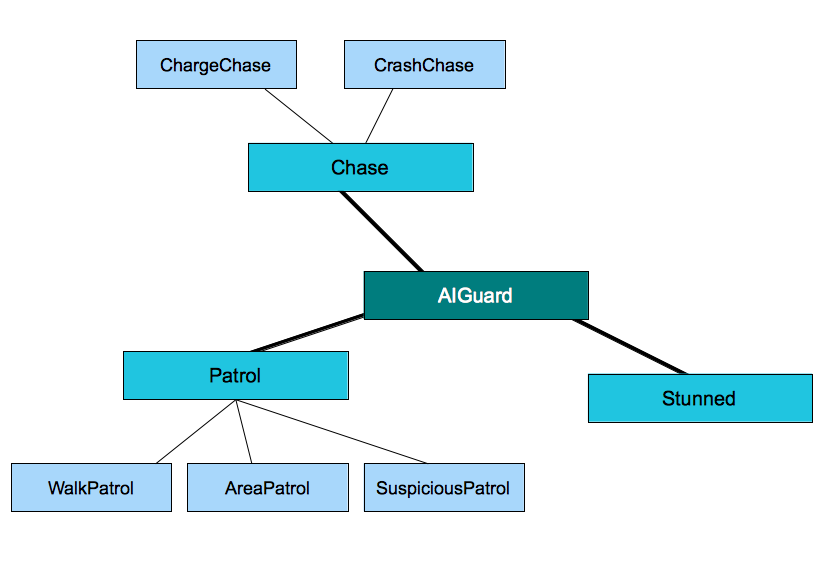
\includegraphics[scale=0.45]{images/development/gerarchiaAIGuard.png}}
\caption{Gerarchia macchina a stati del nemico ``Guard''.}
\label{fig:gerarchiaAIGuard}
\end{figure}

Infine, diciamo che correlato ai nemici, c'è lo script che gestisce la loro generazione, chiamato \manclass{spawner}. Questo genera da 1 ad ``n'' nemici, ad un ritmo di ``tot'' secondi (personalizzabile anche questo), avendo cura di controllare quanti nemici generati siano ancora in vita, così da non sforare il limite massimo scelto. Quando un nemico muore, se generato da uno spawner, richiama un metodo dell'istanza del relativo \manclass{spawner}, avvisando che è morto, quindi decrementando il contatore interno di nemici in vita.

\section{Menù, schede informative e contenuti sbloccabili}

Sia il menù di pausa che l'interfaccia utente delle schede informative, sono state implementate tramite l'uso della ``UI'' di Unity3d, un componente dell'editor Unity aggiunto nella versione 4.6. Gli script che regolano l'uso sono rispettivamente \manclass{MenuManager} e \manclass{InformativeManager}. Il primo gestisce il menù di pausa, mentre il secondo la navigazione dei contenuti Serious del gioco (oltre che metodi per analizzare quanto i contenuti siano stati letti, ma di questo parleremo nella sezione \ref{analisiFruizione}). 

Quando si entra in pausa, il timeScale passa a zero (una proprietà di Unity che regola lo scorrere del tempo) e si tiene traccia che non si è in gioco anche tramite una variabile statica della classe \manclass{PlayStatusTracker}, ``inPlay'', se questa è true, è attivo o il menù o l'interfaccia delle schede informative.
Il menù da la possibilità di ricominciare il livello, uscire dal gioco (e accedere alla prima scena con il menù principale) e accedere alle schede informative. 

La sezione di schede informative, come descritto nella sezione di design (\ref{chap:game_design}), è navigabile in modo da accedere a vari contenuti con le relative immagini. Lo sblocco di un contenuto, avviene tramite lo script \manclass{UnlockContent}, il quale comunica ad \manclass{InformativeManager} quale contenuto è stato sbloccato.

\section{UI in-game}

Le classi \textit{PlayingUI} e \textit{PlayingUILateral} si occupano di fornire dei metodi di accesso agli elementi che costituiscono l’interfaccia di gioco.

\textit{PlayingUI} si occupa dei 4 angoli dello schermo. Per ognuno di essi esiste la possibilità di specificare un’immagine o una serie di esse, da poter essere mostrate in verticale o orizzontale.
Le immagini possono quindi essere di tre dimensioni predefinite, così da fornire la possibilità di evidenziare determinati elementi, oltre che accompagnate dalla grafica di un bottone, di dimensioni standard, anche questo posizionabile in basso o lateralmente rispetto alla serie di immagini.
La classe fornisce chiaramente metodi per cambiare immagini, nasconderle, mostrarle ed accedere direttamente agli oggetti che costituiscono l’interfaccia.
Attualmente, nel prototipo sviluppato, viene utilizzata per mostrare in alto a destra il comando da premere per aprire le schede informative, come si può osservare in Figura~\ref{fig:interfaccia_ingame} e per mostrare al giocatore il vetrino attualmente utilizzabile dalla Lanterna Magica.

\textit{PlayingUILateral} invece, offre metodi simili a quelli di \textit{PlayingUI}, con la differenza data dal fatto che si occupa principalmente di gestire le sezioni laterali dell’interfaccia di gioco.
Permette quindi di creare due serie di immagini a destra ed a sinistra dello schermo, inserite in una barra che funge da contenitore. Questi insiemi di oggetti possono essere quindi mostrati e nascosti dinamicamente.
Attualmente viene utilizzata per mostrare all’utente gli oggetti e le stelle raccolte, rispettivamente nella parte destra e sinistra dello schermo, come mostrato in Figura~\ref{fig:rigiocabilita_UI_hub}.


\section{GeneralFinder e Utils}

Sono stati creati degli script per agevolare e rendere più efficiente le varie logiche di gioco. Per esempio, è stato creato uno script, chiamato \manclass{GeneralFinder} che raccoglie tutti i riferimenti più importanti della scena (come \manclass{PlayerMovements}, \manclass{InformativeManager} etc) e li immagazzina in variabili statiche, in modo che se un qualunque script debba in una qualunque parte del codice, accedere allo script del player, può farlo così: \manclass{GeneralFinder.PlayerMovements}, senza quindi dover cercare ogni volta il GameObject che lo contiene.

L'altro script creato ai fini di un risparmio di codice e resa efficiente del tutto, è \manclass{Utils} il quale implementa delle funzioni simili a quelle della libreria standard di Unity3d, ma dando funzionalità aggiuntive, utili sia per il nostro progetto sia per altri progetti generici.

\subsection{Oggetti interagibili}

La classe \textit{InteragibileObject} si occupa di fornire un’interfaccia standard per tutti gli oggetti dello scenario con cui è possibile interagire. È quindi utilizzata da leve, porte di fine ed inizio livello, oggetti collezionabili, personaggi non giocabili con cui dialogare. Dispone di metodi che mostrano a schermo il comando che il giocatore deve utilizzare per interagire con gli oggetti. Il comando si adatta dinamicamente all’uso o meno del controller.
I metodi di interazione e la grafica del comando da utilizzare vengono mostrati esclusivamente quando il giocatore si trova nei pressi dell’oggetto e scompaiono quando questo si allontana.
Al momento dell’interazione vengono invocati i metodi di oggetti specificati con variabili pubbliche tramite \textit{inspector}.

\subsection{Porte con bottoni}

L'utilizzo di porte che vengono aperte da bottoni avviene frequentemente nel gioco. Il comportamento più usato nel gioco prevede la pressione del bottone e il relativo innalzamento della porta corrispettiva, questa tornerà poi giù quando il bottone verrà rilasciato. Nonostante questo sia l'unico comportamento presente nella demo giocabile, sono state implementate delle varianti per l'apertura delle porte, una per esempio prevede che la porta rimanga alzata anche dopo il rilascio del bottone, oppure un'altra variante ancora prevede che la porta si apra (raggiungendo il suo picco di apertura) fin quando il bottone è premuto, quando invece nella configurazione di default basta toccare anche per un solo istante il bottone per fare aprire completamente la porta. Inoltre la logica prevede la possibilità di unire in serie più porte o meccanismi, sia in traslazione che in rotazione, al fine di risolvere degli enigmi presenti nei livelli di gioco. Sono stati previsti vari modi per premere un bottone, fra i quali, il passaggio del player, quello di un nemico o quello di un oggetto cassa.

\begin{figure}[h]
\centerline{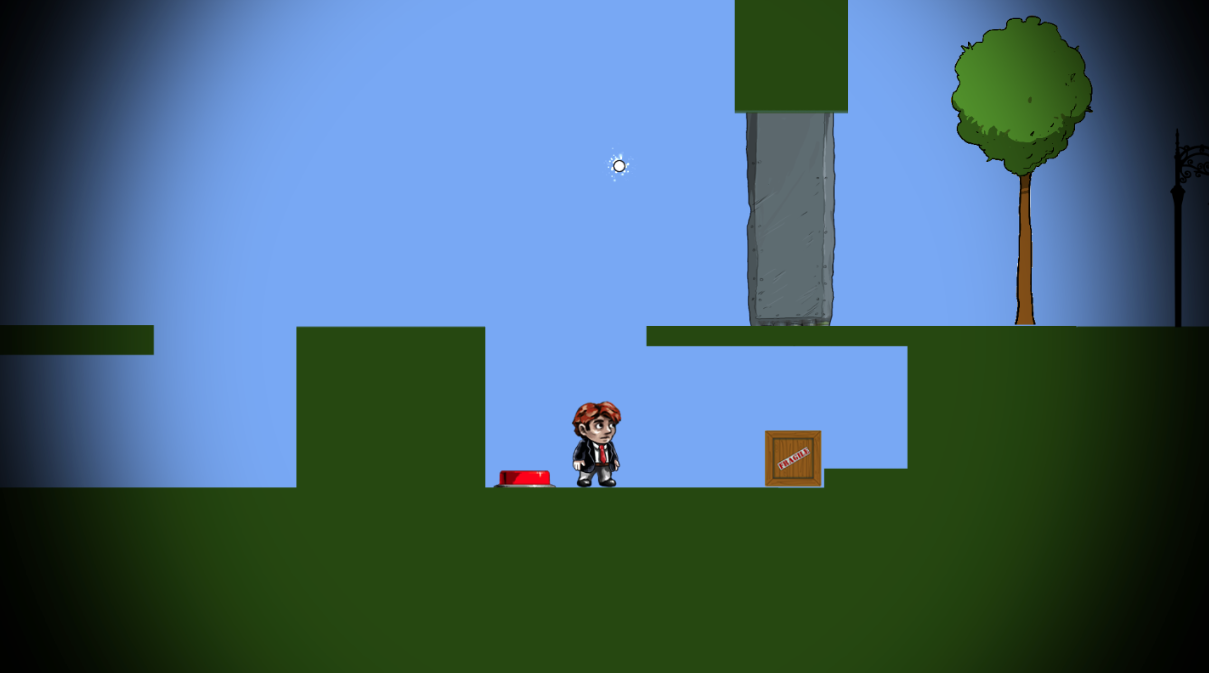
\includegraphics[scale=0.35]{images/development/portaebottone.png}}
\caption{Focus su porta e bottone, dal gameplay di The Magic Lantern.}
\label{fig:portaebottone}
\end{figure}

%\subsection{Camera}

%\subsection{Altro...}

\section{Strumenti per il testing}

\subsection{Analisi di gameplay}
\label{sec:analisi_gamplay}

Durante lo sviluppo è risultato fondamentale studiare metodi efficaci per analizzare il gameplay dei giocatori e dei tester con strumenti oggettivi che ci avessero permesso di ricavare utili statistiche, ai fini di revisione del design e delle soluzioni applicate.
Abbiamo perciò sviluppato alcuni strumenti che ci avessero fornito informazioni riguardo:

\begin{itemize}
	\item Tempo trascorso in ogni porzione di livello.
	\item Game Over del personaggio.
	\item Equilibrio e organizzazione del Level Design.
	\item Difficoltà del gioco.	
\end{itemize}

Di seguito vengono quindi trattate alcune classi sviluppate appositamente per gli scopi appena esposti, con l’aggiunta di un sistema di replay della partita.

\paragraph{ZoneAnalyzer.}
\label{par:zone_analyzer}
È una classe che si occupa di salvare su file i dati relativi al tempo trascorso dal giocatore in ogni sezione di gioco. Il suo comportamento può essere quello di \textit{colelctor} o \textit{analyzer}. Ogni analyzer sfrutta uno o più collider di tipo \textit{trigger} che delimitano la porzione di gioco da analizzare. Quando il personaggio si trova all’interno della zona, viene incrementata una variabile che tiene conto del tempo trascorso. In ogni scena esiste un solo collector, che si occupa invece, al momento della chiusura del livello o del gioco, di raccogliere i dati di tutti gli analyzer e salvarli in un file .xml. Inoltre, ogni volta che il personaggio va in Game Over, lo script \textit{playerMovements} invia un messaggio che specifica il tag dell’oggetto che ha ucciso il player. In questo modo, si può tenere traccia, per ogni zona, del numero di morti generate da:

\begin{itemize}
	\item Nemici.
	\item Punte infilzanti.
	\item Porte.
\end{itemize}

\paragraph{HintAnalyzer.}
\label{par:hint_analyzer}
Si occupa di salvare su file .xml il numero di utilizzi di ogni aiuto usato nel gioco. Esistono alcuni trigger, in varie sezioni di gioco, che, nel caso il personaggio rimanga per troppo tempo al loro interno, fanno comparire un aiuto che permette al giocatore di non rimanere bloccato. Ogni volta che un aiuto viene attivato, la classe \textit{TutorialHInt}, che si occupa di gestirli, invia un messaggio all’HintAnalyzer, che riesce quindi a tener conto delle volte che il giocatore ha fatto uso di aiuti. Questa classe ci fa capire se il bilanciamento della curva di difficoltà è adeguato o meno.

\paragraph{SpikesAnalyzer.}
\label{par:spikes_analyzer}
Classe sviluppata inizialmente per calcolare il numero di morti dovute a punte infilzanti. In seguito all’ampliamento della classe \textit{ZoneAnalyzer}, è stata utilizzata soprattutto per verificare la difficoltà dei salti. Anche questa può avere il comportamento di \textit{analyzer} e \textit{collector}, i primi si occupano di contare il numero di volte in cui il player collide con dei trigger, il collector raccoglie quindi tutti i dati e li salva su .xml. Viene posto un analyzer nella porzione immediatamente sottostante ad un salto, così che, se si notano numeri troppo elevati, significa che il salto era troppo difficile e poco bilanciato.

\paragraph{Sistema di replay.}
\label{par:replay}
È stata appositamente creata la classe \textit{InputKeeper}, che funge da interfaccia per ogni input utilizzato dall’utente. La classe, se appositamente impostato, si occupa di salvare su file ogni variazione sugli input, accompagnandola dal tempo, in secondi, in cui è avvenuta. Con una diversa impostazione, la classe può fare in modo di utilizzare dei dati precedentemente salvati per simulare degli input dell’utente, invece caricati da file. In questo modo è possibile riosservare l’intera partita di un giocatore, e capirne eventuali criticità.

\subsection{Analisi della fruizione di contenuti Serious}
\label{analisiFruizione}

Per capire quanto i contenuti Serious vengano letti o visti dagli utenti, in vista del testing, sono stati usati gli script \manclass{InformativeManager} e \manclass{TestInformativeManager}. Il salvataggio dei dati avviene tramite un xml dove nel quale si serializza la classe \manclass{InfoSectionContainer}, la quale contiene informazioni riguardo i contenuti (\manclass{InformativeContent} e \manclass{SubContent}) e le relative sezioni (\manclass{InformativeSection}).

I dati salvati riguardano:

\begin{itemize}

\item I tempi, oltre che il numero di volte, impiegati per visualizzare una scheda informativa (cioè un contenuto), avendo pure il dettaglio per sotto-contenuto. Si è tenuto traccia pure del fatto che la scheda sia stata aperta o meno una volta sbloccata o se fosse stata vista in un secondo momento.
\item Poiché sono presenti dei quiz durante i livelli (riguardo i contenuti Serious), si è tenuto traccia del numero di tentativi sbagliati e se alla fine si è risposto in modo corretto.

\end{itemize}

\newpage
